% EBMA paper for Political Analysis: Full (unblinded) version 
% Written by: Jacob M. Montgomery, Florian Hollenbach, and Michael
% D. Ward.
% Last update on: 15/12/2011
% Last updated : Florian & Mike


%\documentclass[pdftex,12pt,fullpage,oneside,endnotes]{amsart}
\documentclass[12pt,fullpage,endnotes]{article}

\usepackage{array,amsmath,psfrag,amssymb,subfigure,tabularx}
\usepackage{hyperref,multicol}
\usepackage{pa}
\usepackage{booktabs}
%\usepackage{vmargin,boxedminipage}
\usepackage[usenames]{color}
\usepackage{datetime}
\usepackage{dcolumn}
\usepackage{wrapfig}
\usepackage{setspace}
\usepackage{url}
\usepackage[english]{babel}
\usepackage{times}
\usepackage{multirow}
\usepackage[pdftex]{graphicx}
\usepackage{lscape}
%\usepackage[top=1in,right=1in,left=1in,bottom=1in]{geometry}
\usepackage{array}
\usepackage{booktabs}
\usepackage{hyperref}
\usepackage{endnotes}

%\graphicspath{ Project"/"NSF BMA"/graphics/}} % change to nsf
\newcommand{\note}[1]{\endnote{\doublespacing#1 \vspace{4 mm}}}

\usepackage{natbib}
\bibpunct{(}{)}{;}{a}{}{,}
\bibdata{Flo_Bib}

\newboolean{blind}
\setboolean{blind}{false}


\title{Improving Predictions Using Ensemble \\ Bayesian Model
  Averaging\thanks{For generously sharing their data and models with
    us, we thank Alan Abramowitz, James Campbell, Robert Erikson, Ray
    Fair, Douglas Hibbs, Michael Lewis-Beck, Andrew D. Martin, Kevin
    Quinn, Stephen Shellman, Charles Tien, \& Christopher Wlezien.
    This project was undertaken in the framework of an initiative
    funded by the Information Processing Technology Office of the
    Defense Advanced Research Projects Agency aimed at producing
    models to provide an Integrated Crisis Early Warning Systems
    (ICEWS) for decision makers in the U.S. defense community. The
    holding grant is to the Lockheed Martin Corporation, Contract
    FA8650-07-C-7749. All the bad ideas and mistakes are our own. 
    We especially want to thank Adrian Raftery and Brendan Nyhan for their
    encouragement and feedback as this project evolved. The editor and the reviewers of {\em Political Analysis}
    provided especially salient and important suggestions that substantially improved our research. }}
\author{
Jacob M. Montgomery\\
	Department of Political Science\\
	Washington University in St. Louis\\
	Campus Box 1063, One Brookings Drive\\
	St. Louis, MO, USA, 63130-4899 
	\and
Florian Hollenbach  \\
	Department of Political Science\\
	Duke University\\
	Perkins Hall 326 Box 90204\\
	Durham, NC, USA, 27707-4330
	\and
Michael D. Ward\\
	Department of Political Science\\
	Duke University\\
	Perkins Hall 326 Box 90204\\
	Durham, NC, USA, 27707-4330\\
	corresponding author: michael.d.ward@duke.edu
} 




\date{\today}


\begin{document}

\maketitle
\thispagestyle{empty}
\clearpage
\pagestyle{myheadings}
\markright{Montgomery, Hollenbach, \& Ward\hfill Ensemble BMA\hfill}
\newpage
\singlespacing

\thispagestyle{empty}


\begin{abstract}
\begin{doublespace}
 We present ensemble Bayesian model averaging (EBMA) and illustrate
  its ability to aid scholars in the social sciences to make more
  accurate forecasts of future events.  In essence, EBMA improves
  prediction by pooling information from multiple forecast models to
  generate ensemble predictions similar to a weighted average of
  component forecasts. The weight assigned to each forecast is
  calibrated via its performance in some validation period. The aim is
  not to choose some ``best'' model, but rather to incorporate the
  insights and knowledge implicit in various forecasting efforts via
  statistical postprocessing.  After presenting the method, we show
  that EBMA increases the accuracy of out-of-sample forecasts relative
  to component models in three applied examples: predicting the
  occurrence of insurgencies around the Pacific Rim, forecasting vote
  shares in U.S. presidential elections, and predicting the votes of
  U.S. Supreme Court Justices.
\end{doublespace}
\end{abstract}

\doublespacing
\newpage

%%% Insert all of the main text
\setcounter{page}{1}
\include{EBMASubmissionBody}




%%Bib 
\singlespacing
\bibliographystyle{chicago}
%\bibliography{Flo_Bib,masterEBMA}
\bibliography{Flo_Bib}

\theendnotes

\newpage

\listoffigures

\begin{table}[p]
\small
% latex table generated in R 2.14.0 by xtable 1.6-0 package
% Tue Dec 20 09:55:28 2011
\begin{center}
  \caption{\footnotesize Validation-period results (2008-2009).  The
    table shows estimated model weights, parameters, and fit
    statistics for the EBMA deterministic forecast and all component
    forecasts of insurgency in 29 countries of the US Pacific Command.  EBMA
    outperforms any single model on most measures.}\label{InSam1}
\begin{tabular}{lrrrrrrrrr}
  \toprule
 & Weight & Constant & Predictor & AUC & PRE & Brier & \% Correct \\ 
  \midrule
LMER & 0.85 & -1.89 & 2.58 & 0.97 & -0.58 & 0.08 & 87.07 \\
   SAE & 0.14 & -1.25 & 3.11 & 0.92 & -0.21 & 0.07 & 90.09\\
 GLM & 0.00 & -1.76 & 1.42 & 0.66 & 0.00 & 0.08 & 91.81 \\
  EBMA &  &  &  & 0.96 & 0.65 & 0.04 & 97.13 \\   
%LMER  & 0.719 &  $-$2.043 &     2.703 & 0.965 &$-$0.421& 0.088 &      88.4  \\
%SAE&   0.281&   $-$0.919&     3.953& 0.936& $-$0.158& 0.053&      90.5       \\
%GLM   &0.000 &  $-$1.760     &1.420 &0.656  &0.000 &0.077&      91.8       \\
%EBMA   & & & &0.959  &0.614 &0.036      &96.8       \\
\bottomrule
 % SAE & 0.57 & 0.04 & 7.46 & 0.96 & 0.48 & 0.04 & 94.11\\ 
 %  LMER & 0.43 & 6.08 & 28.25 & 0.96 & 0.01 & 0.07 & 88.79\\ 
 %  GLM & 0.00 & 0.57 & 8.16 & 0.65 & 0.00 & 0.10 & 88.65\\ 
 %  EBMA &  &  &  & 0.97 & 0.55 & 0.04 & 94.94\\ 
 %   \bottomrule
n=696\\
\end{tabular}
\end{center}
\end{table}


\begin{table}[p]
\small
\begin{center}
  \caption{\footnotesize Test-period results (2010).  The table shows
    fit statistics for the EBMA deterministic forecast and all
    component model forecasts of insurgency in 29 countries of the
    Pacific Rim for the test-period.  EBMA equals or outperforms any single model on all
    measures.}\label{OutSam1}
\begin{tabular}{lrrrrr}
  \toprule
 & AUC & PRE & Brier & \% Correct   \\ 
  \midrule
LMER & 0.97 & 0.11 & 0.08 & 91.09\\
SAE  & 0.96 & 0.20 & 0.06 & 91.95\\
GLM & 0.72 & 0.00 & 0.09 & 89.94\\
EBMA & 0.97 & 0.43 & 0.04 & 94.25 \\
%LMER  &0.971& 0.114& 0.084&      91.1\\
%SAE & 0.972& 0.143& 0.046&      91.4\\
%GLM& 0.721& 0.000& 0.088&      89.9\\
%EBMA &0.979& 0.371& 0.037&      93.7\\
 % SAE &  0.96 & 0.04 & 0.06 & 89.80   \\ 
  % LMER & 0.97 & 0.00 & 0.07 & 89.37  \\ 
  % GLM & 0.84 & 0.00 & 0.09 & 89.37  \\ 
  % EBMA & 0.96 & 0.18 & 0.05 & 91.24 \\ 
   \bottomrule
n=348 \\
\end{tabular}
\end{center}
\end{table}

\begin{table}[p]
  \caption{\footnotesize Test-period prediction errors, model weights, and validation-period fit 
    statistics for component and EBMA forecasts  of the 2004 and 2008  
    elections. The models are trained using \textit{all} prior data and the 
    EBMA model is validated on the observations beginning in 1952.  
    The EBMA model does better than all components on 
    validation-sample fit statistics.  In addition, although it does not 
    necessarily make the most accurate prediction for any given year,
    it is less likely to make  dramatic forecasting errors for the test-period.}
\label{Pres-Year-Res} \small
\begin{center}
\begin{tabular}{l rrrrrrrr}	
  \toprule
   &\multicolumn{4}{c}{\textit{2004 Election}} &\multicolumn{4}{c}{\textit{2008 Election}} \\ 
 &	Weights&	RMSE &MAE &\shortstack{Pred. \\ Error}
 &Weights&	RMSE&	MAE &  \shortstack{Pred.\\  Error}\\
\midrule
 Campbell               & 0.40 & 1.71 & 1.33 & 0.53 & 0.36 & 1.65 & 1.28 & 6.33\\
  Abramowitz        	& 0.00 & 1.50 & 1.18 & 2.20 & 0.06 & 1.53 & 1.26 & -2.37\\
  Hibbs                   	& 0.12 & 1.95 & 1.38 & 1.54 & 0.25 & 1.92 & 1.38 & -1.39\\
  Fair                      	& 0.48 & 2.07 & 1.47 & 4.82  & 0.00 & 2.22 & 1.80 & -2.02 \\
  Lewis-Beck/Tien 	& 0.00 & 1.67 & 1.42 & -0.41& 0.17 & 1.61 & 1.33 & -2.64\\
  EWT2C2 		& 0.00 & 2.67 & 2.06 & 4.76  & 0.17 & 2.81 & 2.18 & -0.14\\
   EBMA                    	&  & 1.29 & 1.02 & 2.08 &  & 1.30 & 1.01 & -0.53\\
   % Campbell               &0.40&1.71&1.33 &0.53&0.36&1.65&1.28&6.33\\
  %Abramowitz        	&0.00&1.50&1.18&2.20&0.06&1.53&1.26&$-$2.37\\
  %Hibbs                   	&0.12&1.95&1.38&1.54&0.25&1.92&1.38&$-$1.39\\
  %Fair                      	&0.48&2.07&1.47&4.82&0.00&2.22&1.80&$-$2.02 \\
  %Lewis-Beck/Tien 	&0.00&1.67&1.42&$-$0.41&	0.17&1.61&1.33&$-$2.65\\
  %Erikson/Wlezien 	&0.00&2.67&2.06&4.76&0.17&2.81&2.18&$-$0.14\\
 %  EBMA                    	&	       	&1.29&1.01&2.08&  &1.30&1.01&$-$0.53\\
\bottomrule
\end{tabular}
 \end{center}
 \end{table}

%%%%% table in footnotes would go in here

\begin{table}[p]
  \caption{\footnotesize Fit statistics and observed coverage
    probabilities for sequentially generated test-sample predictions
    of presidential elections from 1976-2008.  EBMA outperforms its
    component models on all metrics.}
\label{Pres-Res} \small
\begin{center}
\begin{tabular}{lrrrrr}
\toprule
                        &              &              & \multicolumn{2}{c}{Coverage} \\ 
                    	&	RMSE&	MAE	&67\% &   90\%      \\
\midrule
Campbell & 2.74 & 1.99 & 0.67 & 0.78 \\ 
  Abramowitz & 2.27 & 2.05 & 0.33 & 0.78 \\ 
  Hibbs & 2.81 & 2.24 & 0.22 & 0.56 \\ 
  Fair & 4.01 & 3.20 & 0.44 & 0.78 \\ 
  Lewis-Beck & 2.27 & 1.82 & 0.89 & 1.00 \\ 
  EWT2C2 & 2.88 & 2.16 & 0.78 & 1.00 \\ 
  EBMA & 1.72 & 1.47 & 0.67 & 0.89 \\
%Campbell	           &	2.74	&	1.99	&	0.67	&	0.78	\\
%Abramowitz	   &	2.27	&	2.05	&	0.33	&     0.78	\\
%Hibbs	           &	2.81	&	2.24	&	0.44&      0.78 \\
%Fair	                   &	4.01	&	3.20	&	0.44	&	0.78	\\
%Lewis-Beck/Tien&	2.27	&	1.82	&	0.89	&	1.00	\\
%Erikson/Wlezien&	2.88	&	2.16	&	0.78	&	1.00	\\
%EBMA	           &	1.72	&	1.47	&	0.67	&	0.89	\\
\bottomrule
\end{tabular}
\end{center}
\end{table}

% latex table generated in R 2.12.0 by xtable 1.5-6 package
% Thu May 12 17:11:59 2011
\begin{table}[p]
  \caption{\footnotesize Test-period results for U.S. Supreme Court
    example.  The table shows fit statistics for the EBMA deterministic
    forecast and component forecasts of U.S. Supreme Court votes on
    cases in the 2002-2003 session with 2002 docket numbers.   EBMA 
    outperforms its component models on all metrics. }
\label{SC-Res} \small
\begin{center}
\begin{tabular}{lrrrrrrr}
\toprule
 & Weight & AUC & PRE & Brier & \% Correct   \\ 
\midrule
MQRK model& 0.32  &0.66 & -0.02 & 0.29 & 70.56  \\ 
Subject experts & 0.68 &0.62 & 0.15 & 0.23 & 75.23 \\ 
EBMA forecast&  & 0.70 & 0.21 & 0.18 & 77.10  \\ 
%MQRK model& 0.32  & 0.66 & -0.02 & 0.29 & 70.56   \\ 
%Subject experts & 0.68 & 0.62 & 0.15 & 0.23 & 75.23  \\ 
%EBMA forecast&  & 0.70 & 0.21 & 0.18 & 77.10  \\ 
\bottomrule
n=214 
\end{tabular}
\end{center}
\end{table}

\clearpage
\begin{figure}[p]
 \caption{\footnotesize Separation plots for validation-period
    predictions of the ICEWS data (n=696).  For each model,
    observations are shown from left to right in order of increasing
    predicted probability of insurgency (shown as the black line).
    Observations where insurgency actually occurred are shown in
    red. EBMA outperforms all component models in assigning high
    predicted probabilities to \textit{more} observed insurgencies and
    to \textit{fewer} non-insurgencies.}
\label{InSam1sep}
\begin{center}
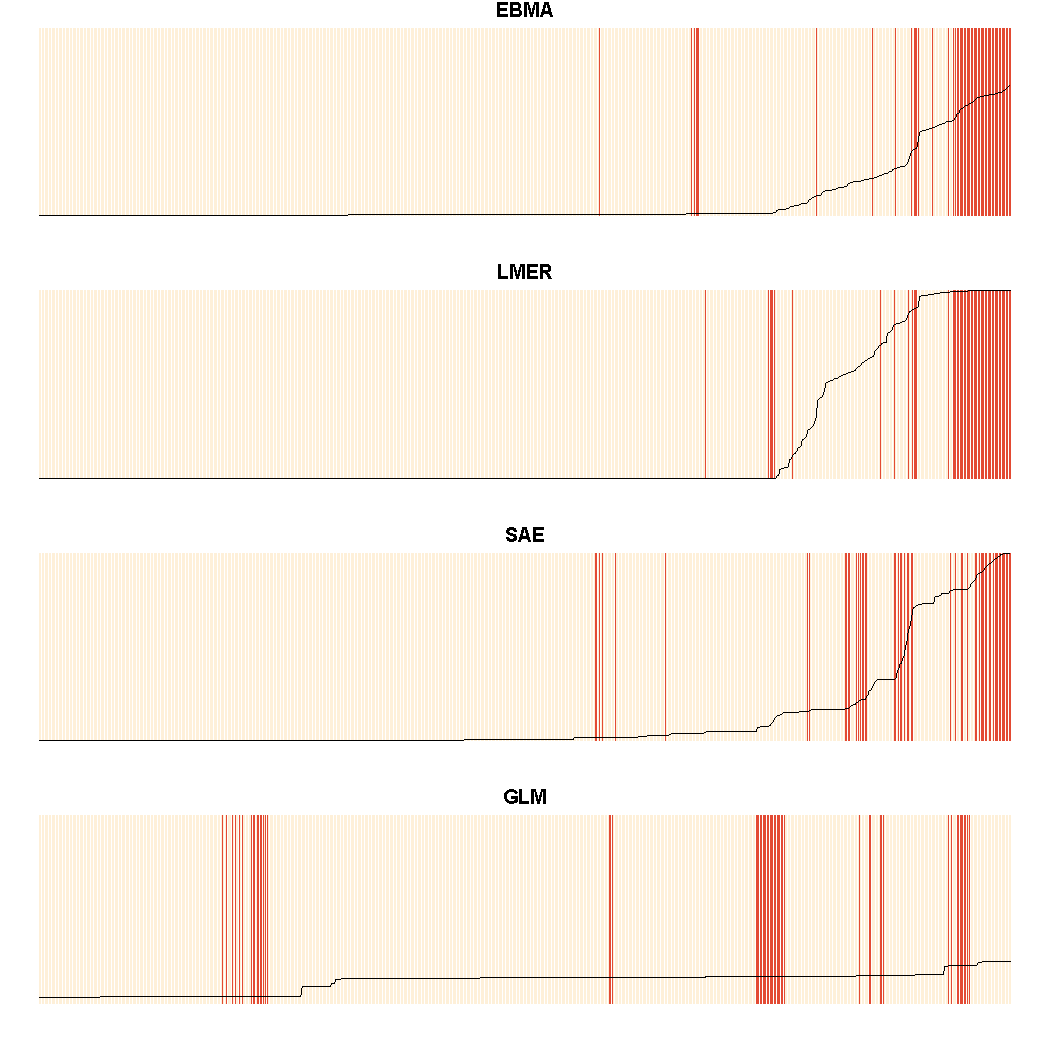
\includegraphics[width=4in]{Insample2-1.pdf}
\end{center}
\end{figure}

\begin{figure}
 \caption{\footnotesize Separation plots for the test-period
    predictions of the ICEWS data (n=348).  For each model,
    observations are shown from left to right in order of increasing
    predicted probability (shown as the black line).  Observations
    where insurgency actually occurred are shown in red.  EBMA
    outperforms all component models in assigning high predicted
    probabilities to \textit{more} observed insurgencies and to
    \textit{fewer} non-insurgencies.}
\label{OutSam1sep}
\begin{center}
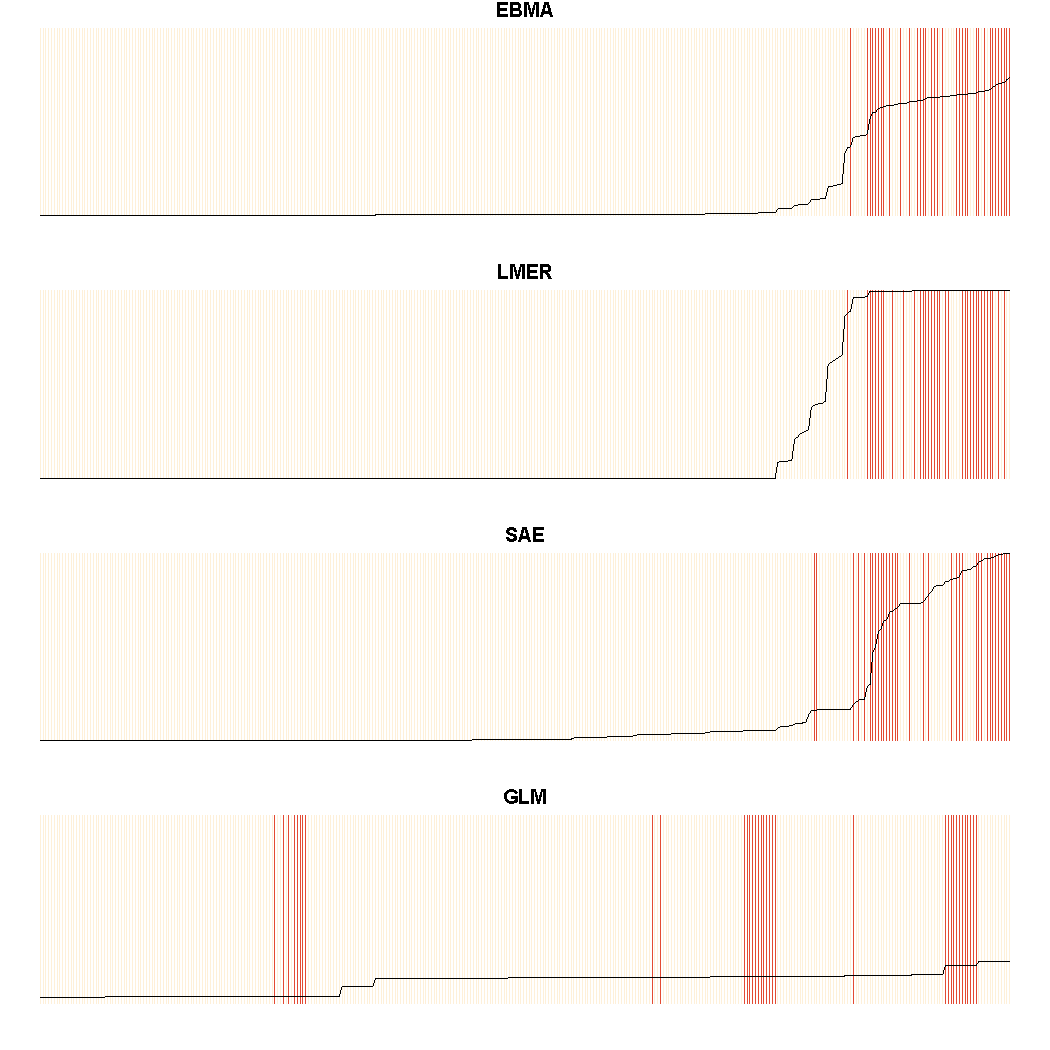
\includegraphics[width=4in]{OutSample2-1.pdf}
\end{center}
\end{figure}


 \begin{figure}[p]
   \caption{\footnotesize The predicted and actual percentage of the
     two-party vote going to the incumbent party in U.S. presidential
     elections from six component models and the EBMA forecast.  For
     each year, the plots show the point predictions (circles), 67\%
     predictive intervals (thick horizontal lines), and 90\%
     predictive intervals (thin horizontal lines).  The vertical
     dashed line is the observed outcome.  The EBMA model is
   better calibrated than its components. }
 \label{PresPlots2}
 \begin{center}
 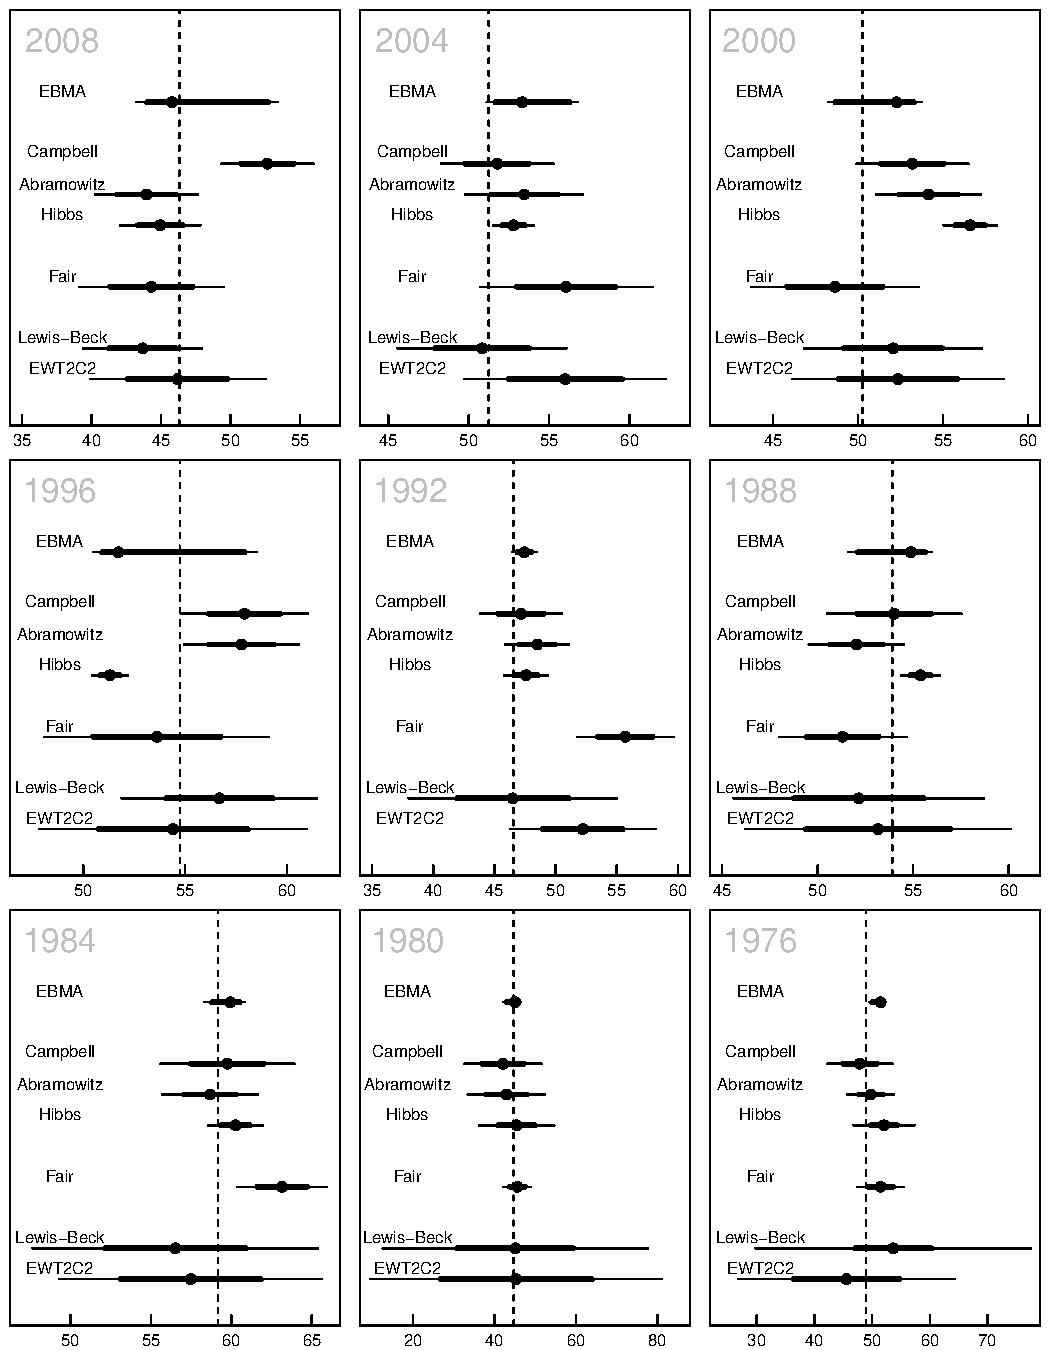
\includegraphics[width=5.6 in]{PresPlot2-1.pdf}
 \end{center}
 \end{figure}




%\bibdata{"Volumes/"ICEWS Project"/"NSF BMA"/flo_Bib","/Volumes/"ICEWS Project"/"NSF BMA"/masterEBMA"}
%\bibliography{/Users/mw160/Documents/BIBTEXFILES/predictionrefs/predictions2,/Users/mw160/Documents/BIBTEXFILES/2009mdwbib}}



%Contact information for authors:

\end{document}
\bye
